\documentclass[a4paper, 14pt]{article}
\usepackage{comment}

\usepackage{setspace}
\usepackage{indentfirst}
%% Language and font encodings
\usepackage{extsizes}
\usepackage[english, russian, ukrainian]{babel}
\usepackage[utf8x]{inputenc}
\usepackage[T1]{fontenc}
\linespread{1.6}
%% Sets page size and margins
\usepackage[a4paper,top=2cm,bottom=2cm,left=3cm,right=2cm,marginparwidth=1.75cm]{geometry}

%\usepackage{fontspec}

%% Useful packages
\usepackage{authblk}
\usepackage{amsmath}
\usepackage{graphicx}
\usepackage[colorinlistoftodos]{todonotes}
\usepackage[colorlinks=true, allcolors=black]{hyperref}
\usepackage{tikz}
%\usepackage{subfigure}
\usepackage[lofdepth,lotdepth]{subfig}
\usepackage{float}
\usepackage{multirow}
\usepackage{hhline}
\usepackage{lineno}

%\linenumbers
\renewcommand{\thefigure}{\thesection.\arabic{figure}}

\numberwithin{equation}{section}
\numberwithin{table}{section}

\title{}


\author[1]{V. Haponov}
\author[2]{R. Yermolenko}
\affil[1]{Taras Shevchenko National University of Kiev, Kiev, Ukraine}
\affil[2]{}

\setcounter{Maxaffil}{0}
\renewcommand\Affilfont{\itshape\normalsize}
\renewcommand{\arraystretch}{1.5} %% increase table row spacing
%\renewcommand{\tabcolsep}{1cm}\documentclass[a4paper, 14pt]{article}
\usepackage{comment}

\usepackage{setspace}
\usepackage{indentfirst}
%% Language and font encodings
\usepackage{extsizes}
\usepackage[english, russian, ukrainian]{babel}
\usepackage[utf8x]{inputenc}
\usepackage[T1]{fontenc}
\linespread{1.6}
%% Sets page size and margins
\usepackage[a4paper,top=2cm,bottom=2cm,left=3cm,right=2cm,marginparwidth=1.75cm]{geometry}

%\usepackage{fontspec}

%% Useful packages
\usepackage{authblk}
\usepackage{amsmath}
\usepackage{graphicx}
\usepackage[colorinlistoftodos]{todonotes}
\usepackage[colorlinks=true, allcolors=black]{hyperref}
\usepackage{tikz}
%\usepackage{subfigure}
\usepackage[lofdepth,lotdepth]{subfig}
\usepackage{float}
\usepackage{multirow}
\usepackage{hhline}
\usepackage{lineno}

%\linenumbers
\renewcommand{\thefigure}{\thesection.\arabic{figure}}

\numberwithin{equation}{section}
\numberwithin{table}{section}

\title{}


\author[1]{V. Haponov}
\author[2]{R. Yermolenko}
\affil[1]{Taras Shevchenko National University of Kiev, Kiev, Ukraine}
\affil[2]{}

\setcounter{Maxaffil}{0}
\renewcommand\Affilfont{\itshape\normalsize}
\renewcommand{\arraystretch}{1.5} %% increase table row spacing
%\renewcommand{\tabcolsep}{1cm}

\begin{document}
	
	\section{Спектри гірчичного газу}
	
		\begin{figure}[hbt!]
			%\vspace{-10pt}
			\centering 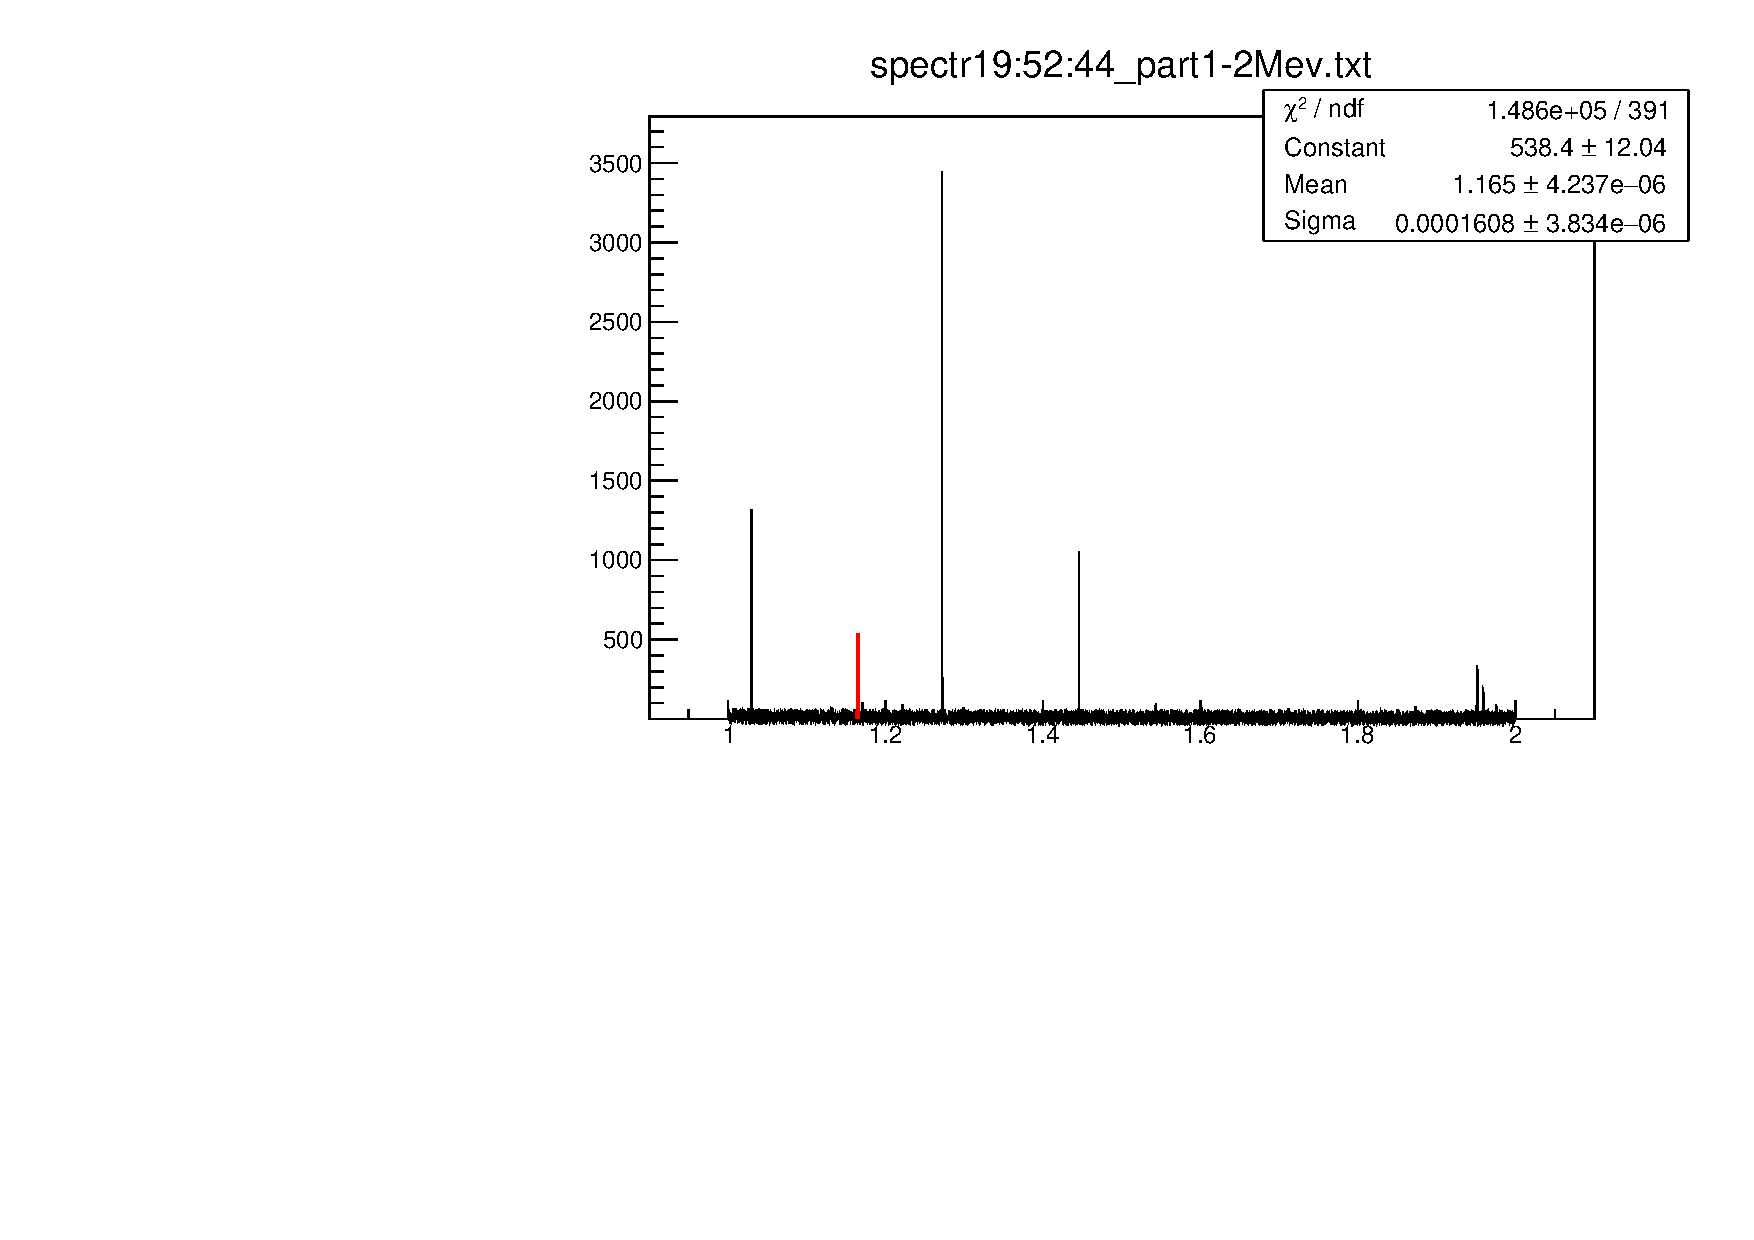
\includegraphics[width=1\textwidth]{Cl1_17.pdf}
			\caption{Fit - ROOT gauss, Лінія яка відповідає 1.17 Mev Cl в проекті Сабат, виділена червоним}
			\label{ris:image1}
		\end{figure}
	
		\begin{figure}[hbt!]
			%\vspace{-10pt}
			\centering 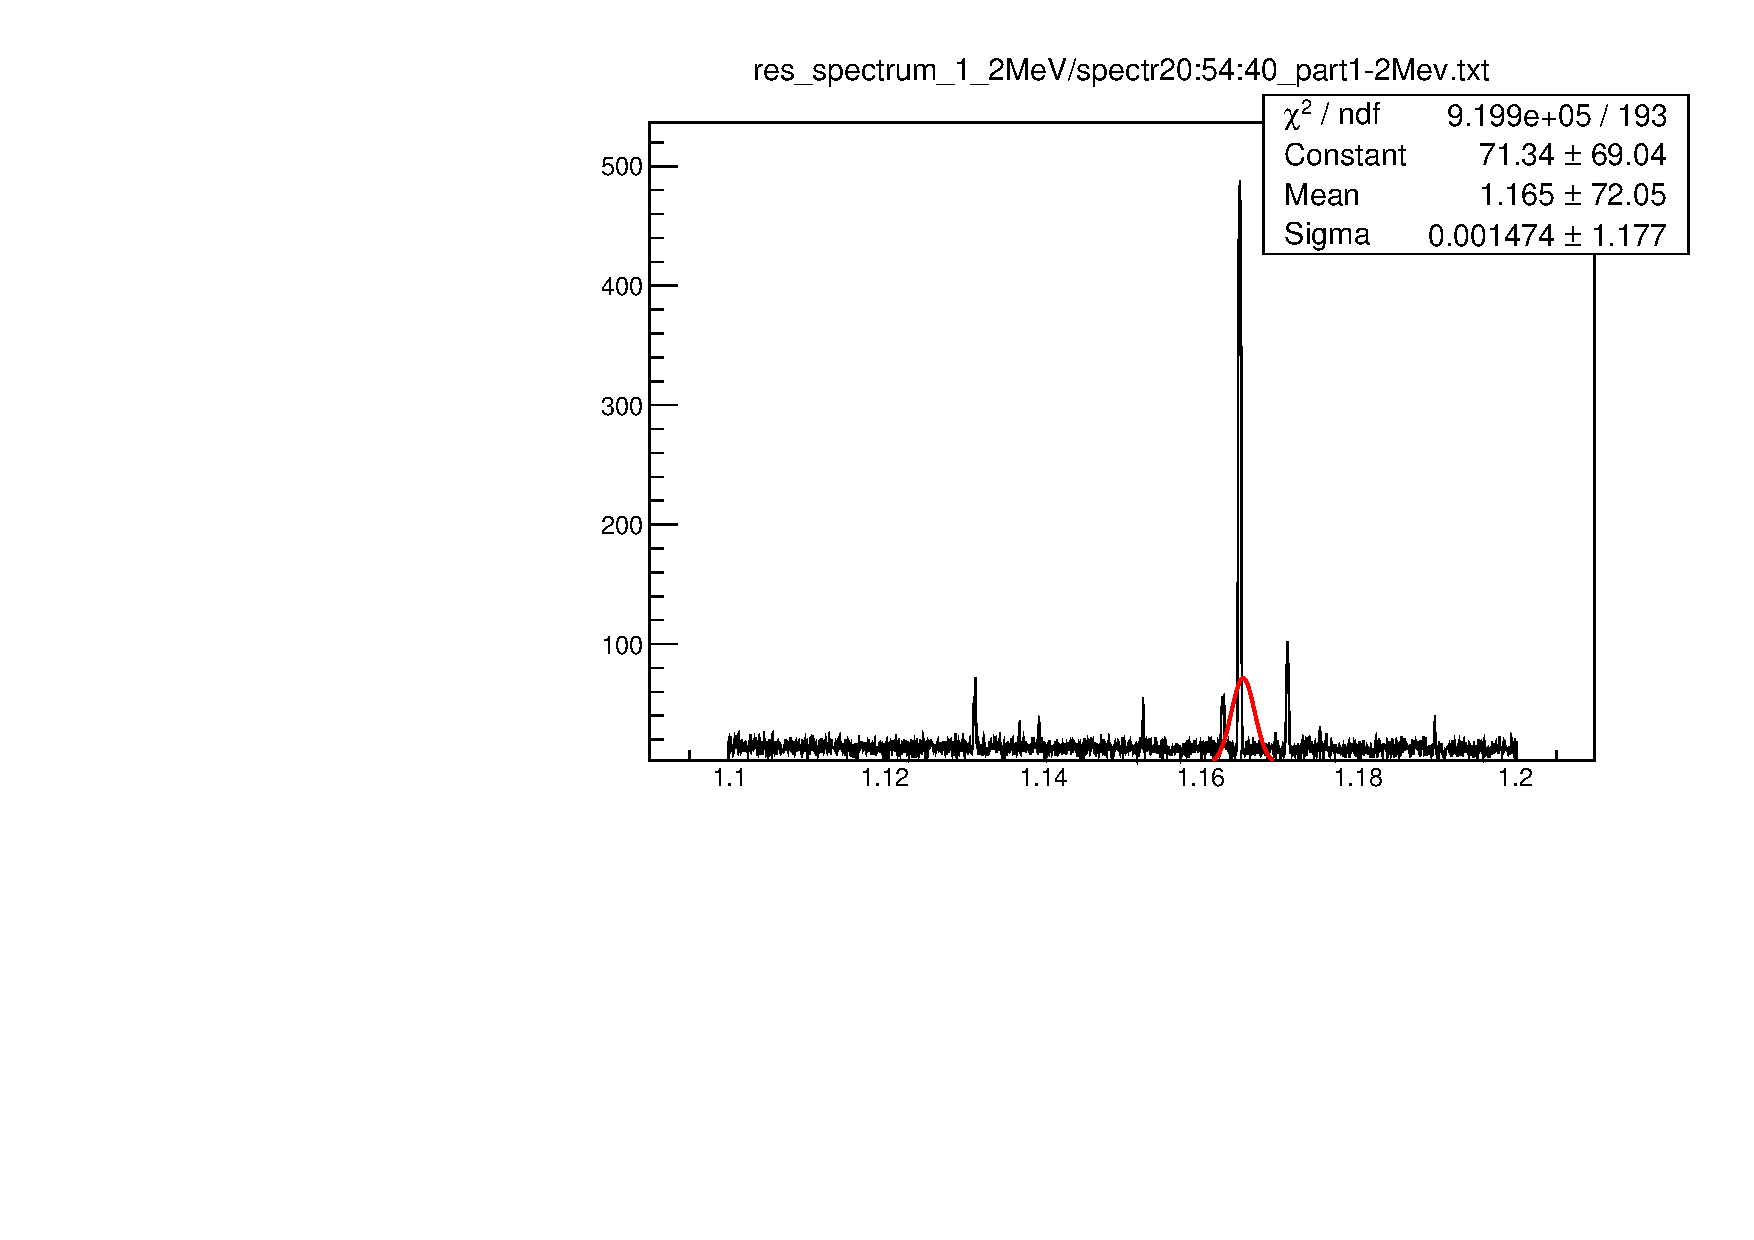
\includegraphics[width=1\textwidth]{Cl_1_17M.pdf}
			\caption{. Fit - ROOT gauss, Лінія яка відповідає 1.17 Mev Cl в проекті Сабат, червоним виділена апроксимація гауссом, маштаб від 1.1MeV - 1.2MeV}
			\label{ris:image2}
		\end{figure}
	
		\begin{figure}[hbt!]
			%\vspace{-10pt}
			\centering 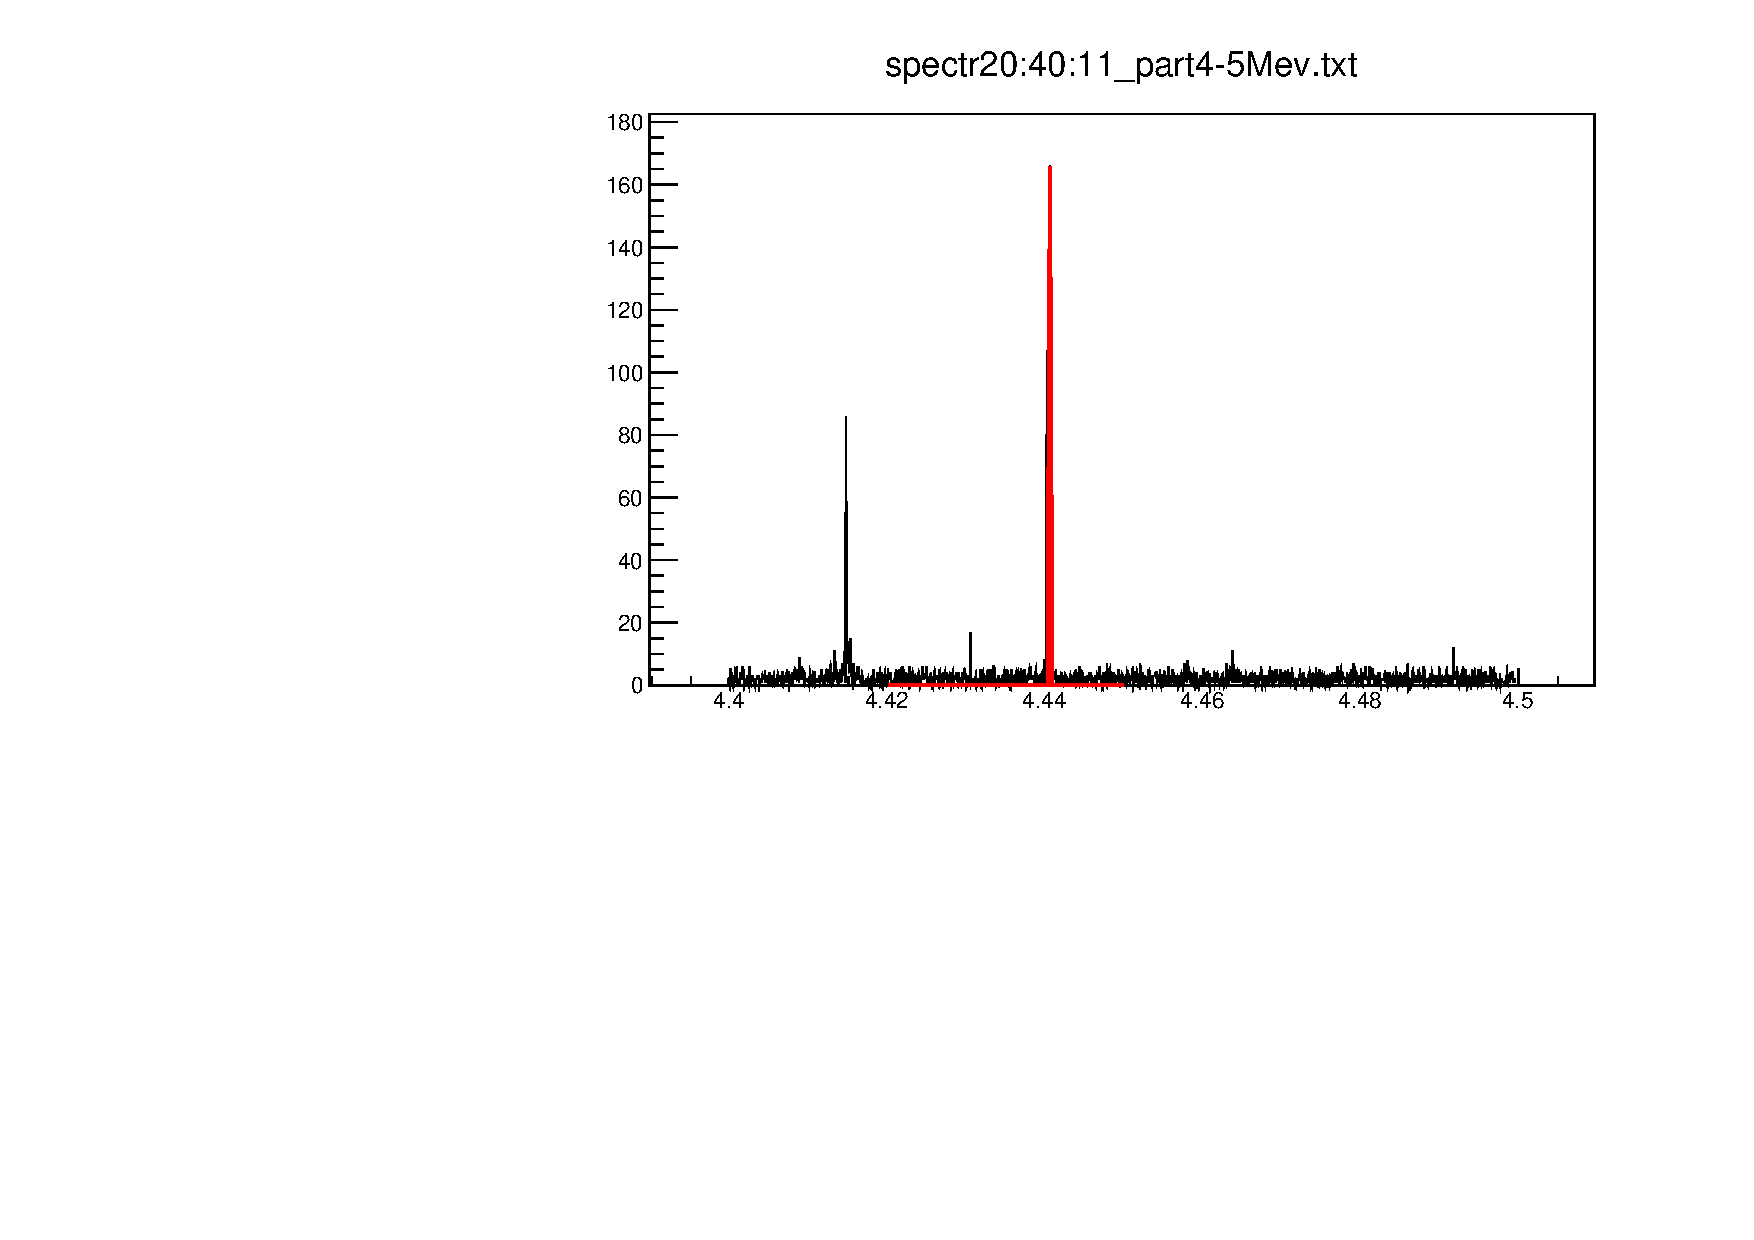
\includegraphics[width=1\textwidth]{C.pdf}
			\caption{Лінія яка відповідає 4.44 Mev C в проекті Сабат, червоним побудований гаусс}
			\label{ris:image3}
		\end{figure}
	
		\begin{figure}[hbt!]
			%\vspace{-10pt}
			\centering 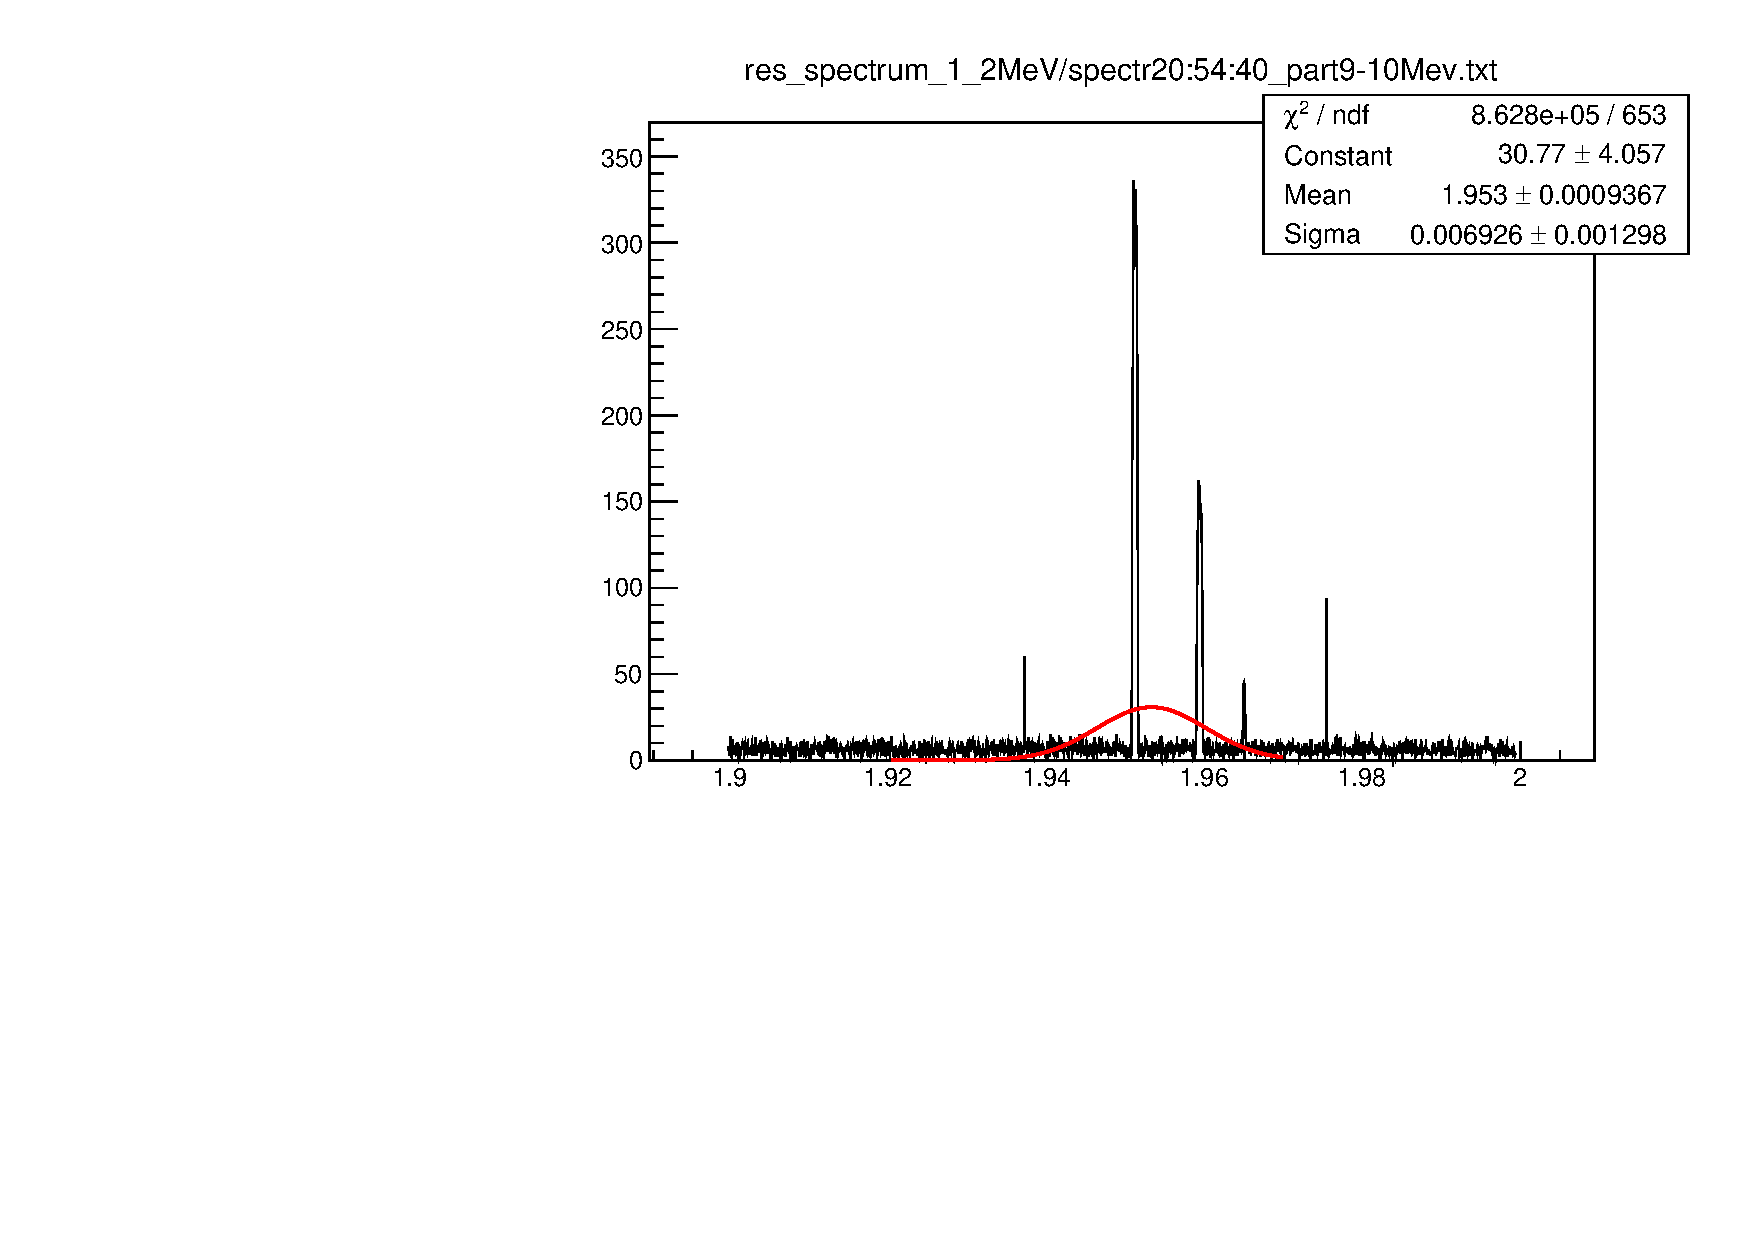
\includegraphics[width=1\textwidth]{Cl_1_94.pdf}
			\caption{Лінія яка відповідає 1.94 Mev Cl в проекті Сабат, червоним побудований гаусс}
			\label{ris:image4}
		\end{figure}

		\begin{figure}[hbt!]
			%\vspace{-10pt}
			\centering 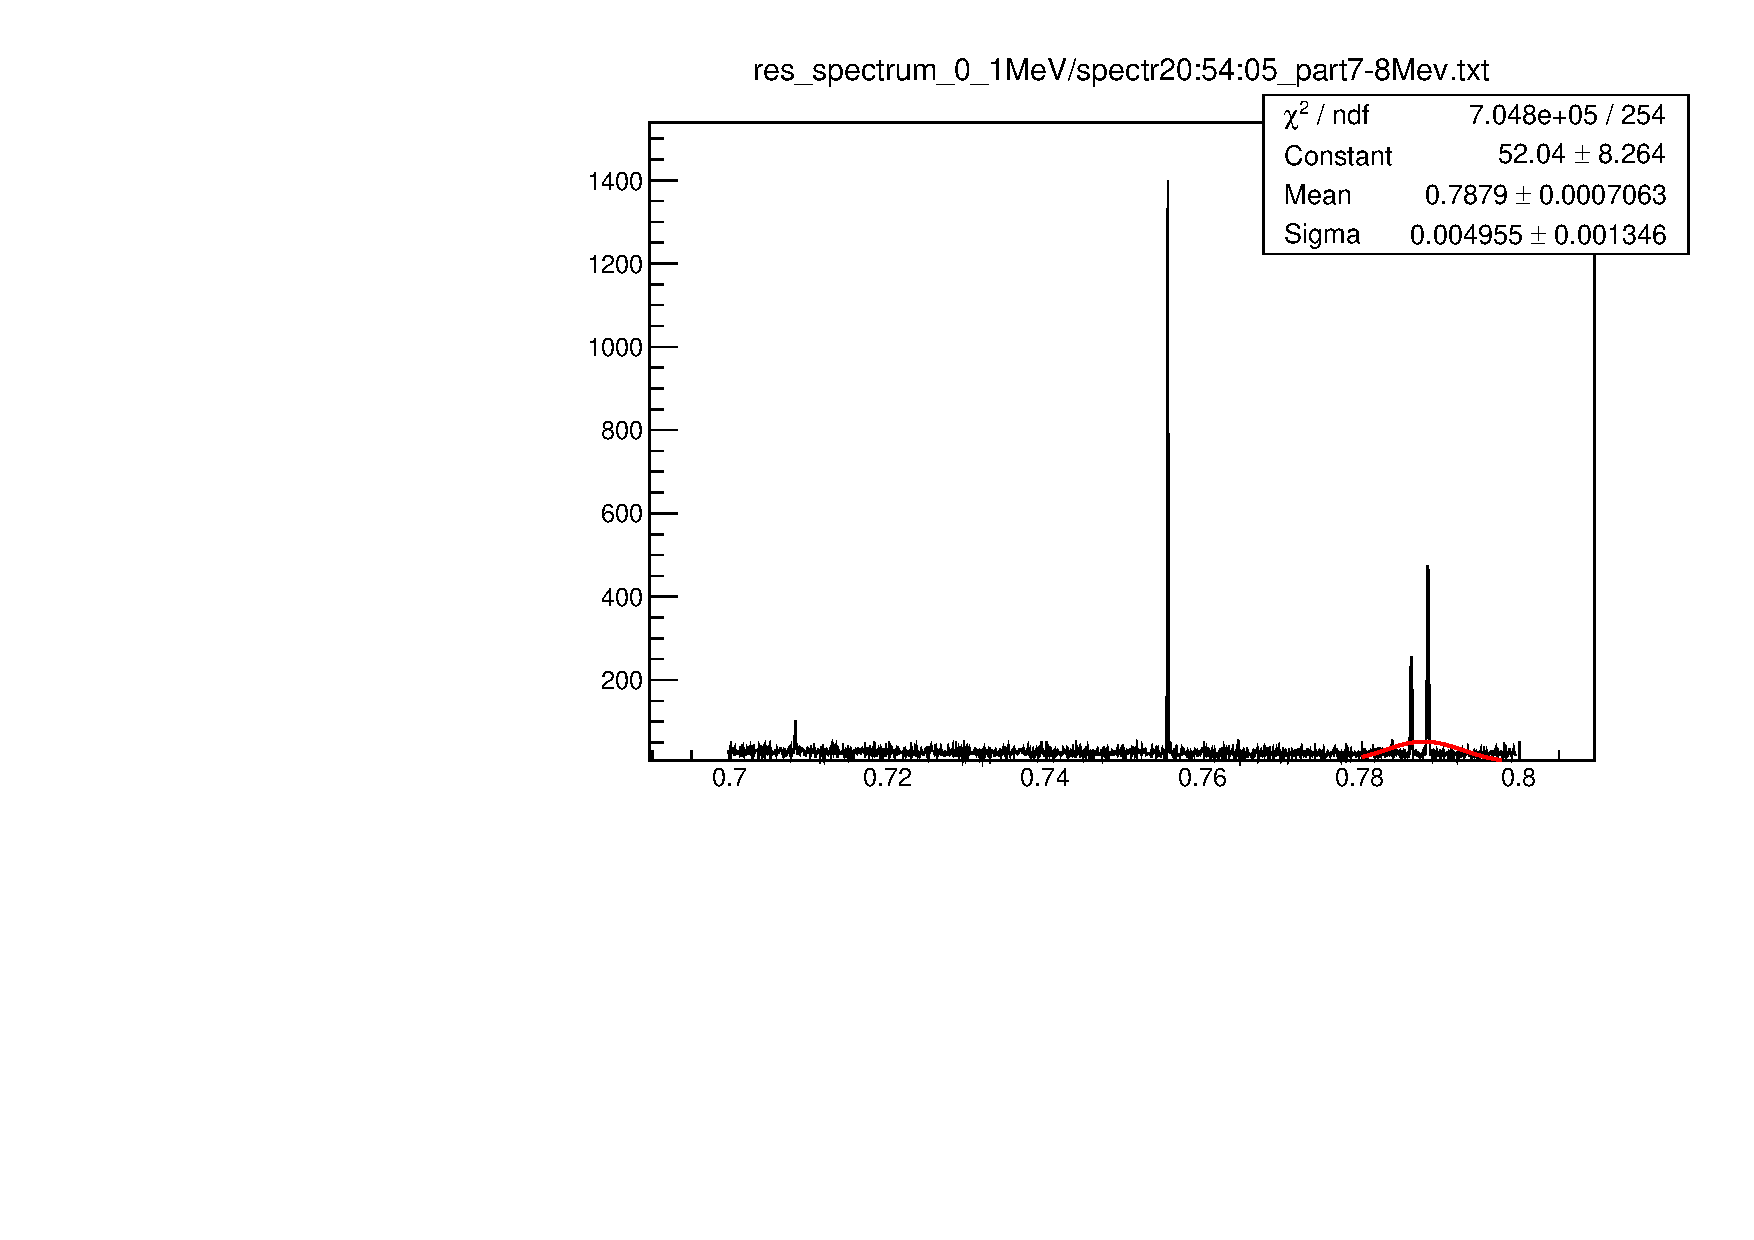
\includegraphics[width=1\textwidth]{Cl_0_79.pdf}
			\caption{Лінія яка відповідає 0.79 Mev Cl в проекті Сабат, червоним побудований гаусс}
			\label{ris:image5}
		\end{figure}
	
		\begin{figure}[hbt!]
			%\vspace{-10pt}
			\centering 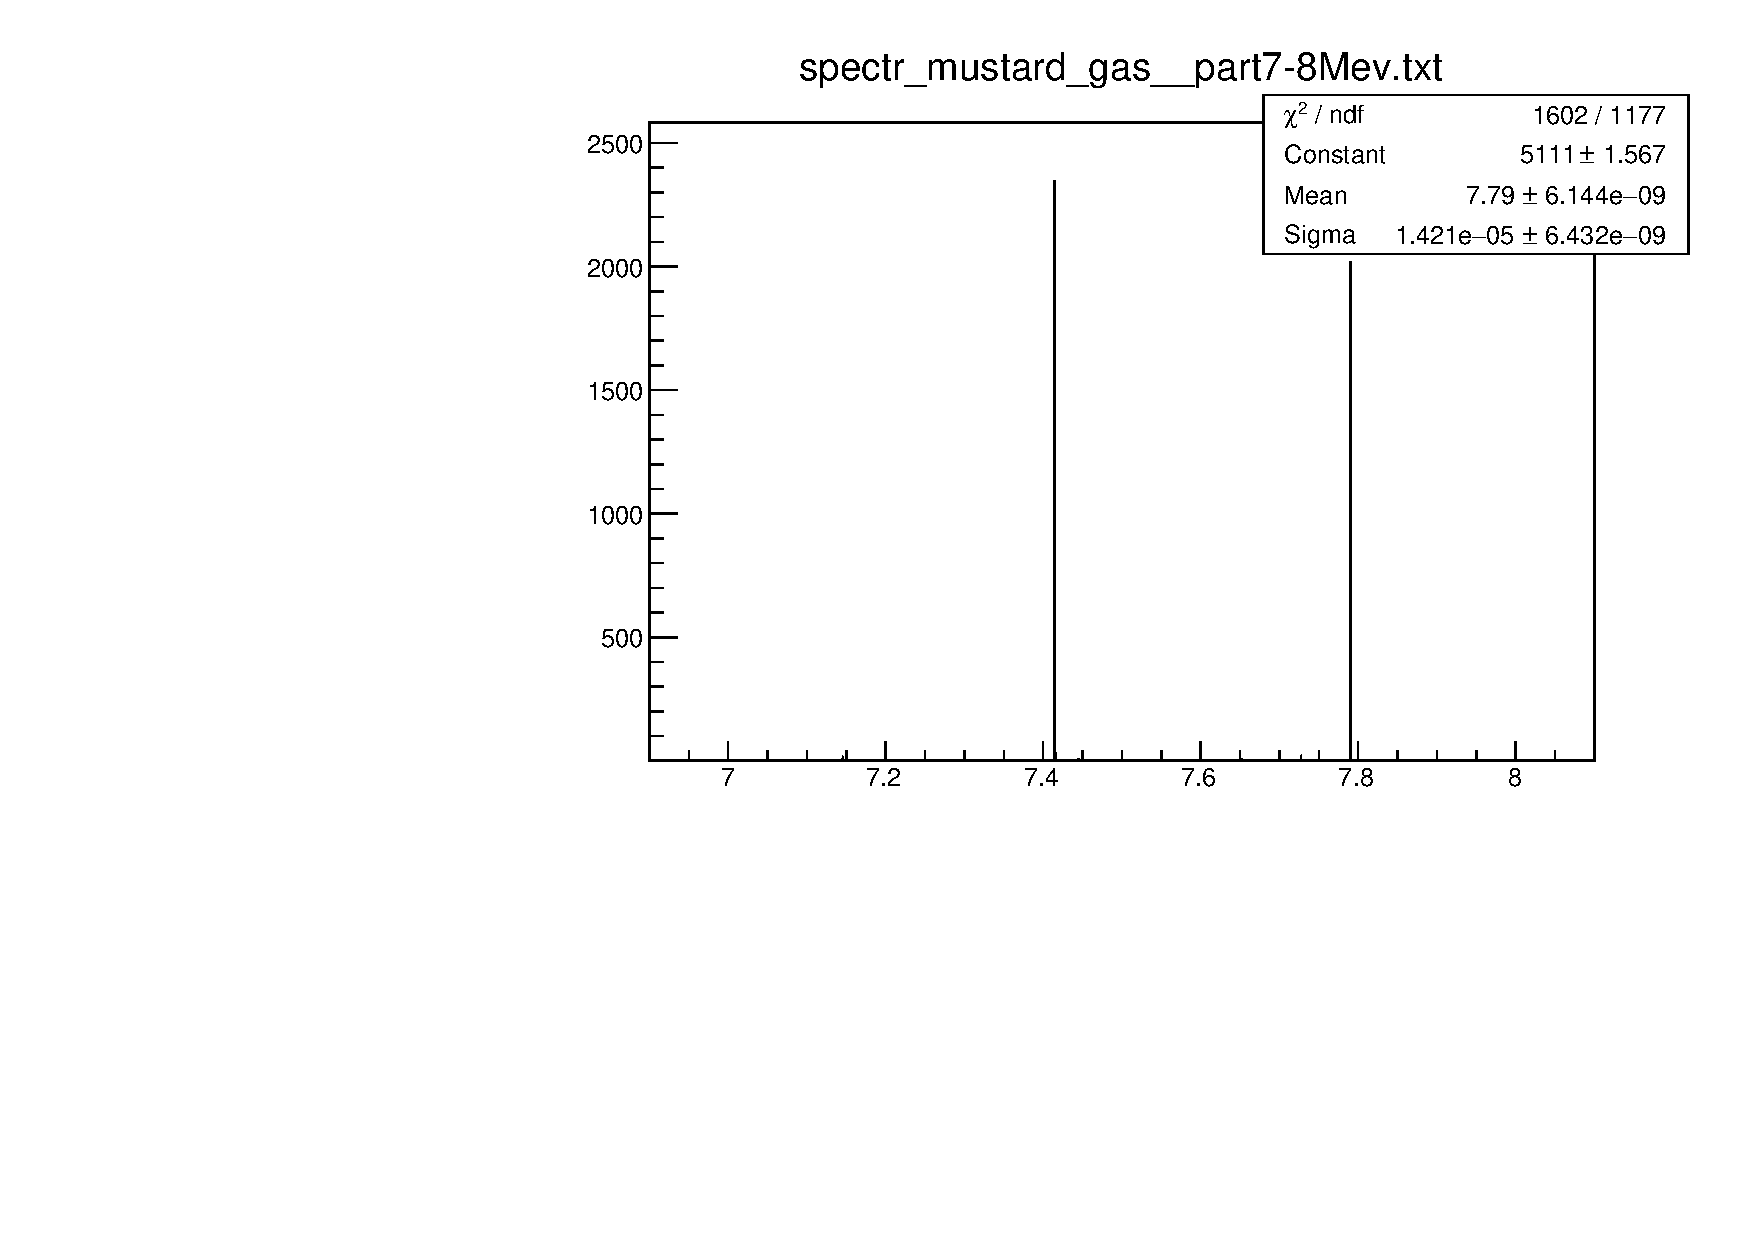
\includegraphics[width=1\textwidth]{Cl7_79MeV.pdf}
			\caption{Лінія яка відповідає 7.79 Mev Cl в проекті Сабат, червоним побудований гаусс}
			\label{ris:image6}
		\end{figure}
	
		\begin{figure}[hbt!]
			%\vspace{-10pt}
			\centering 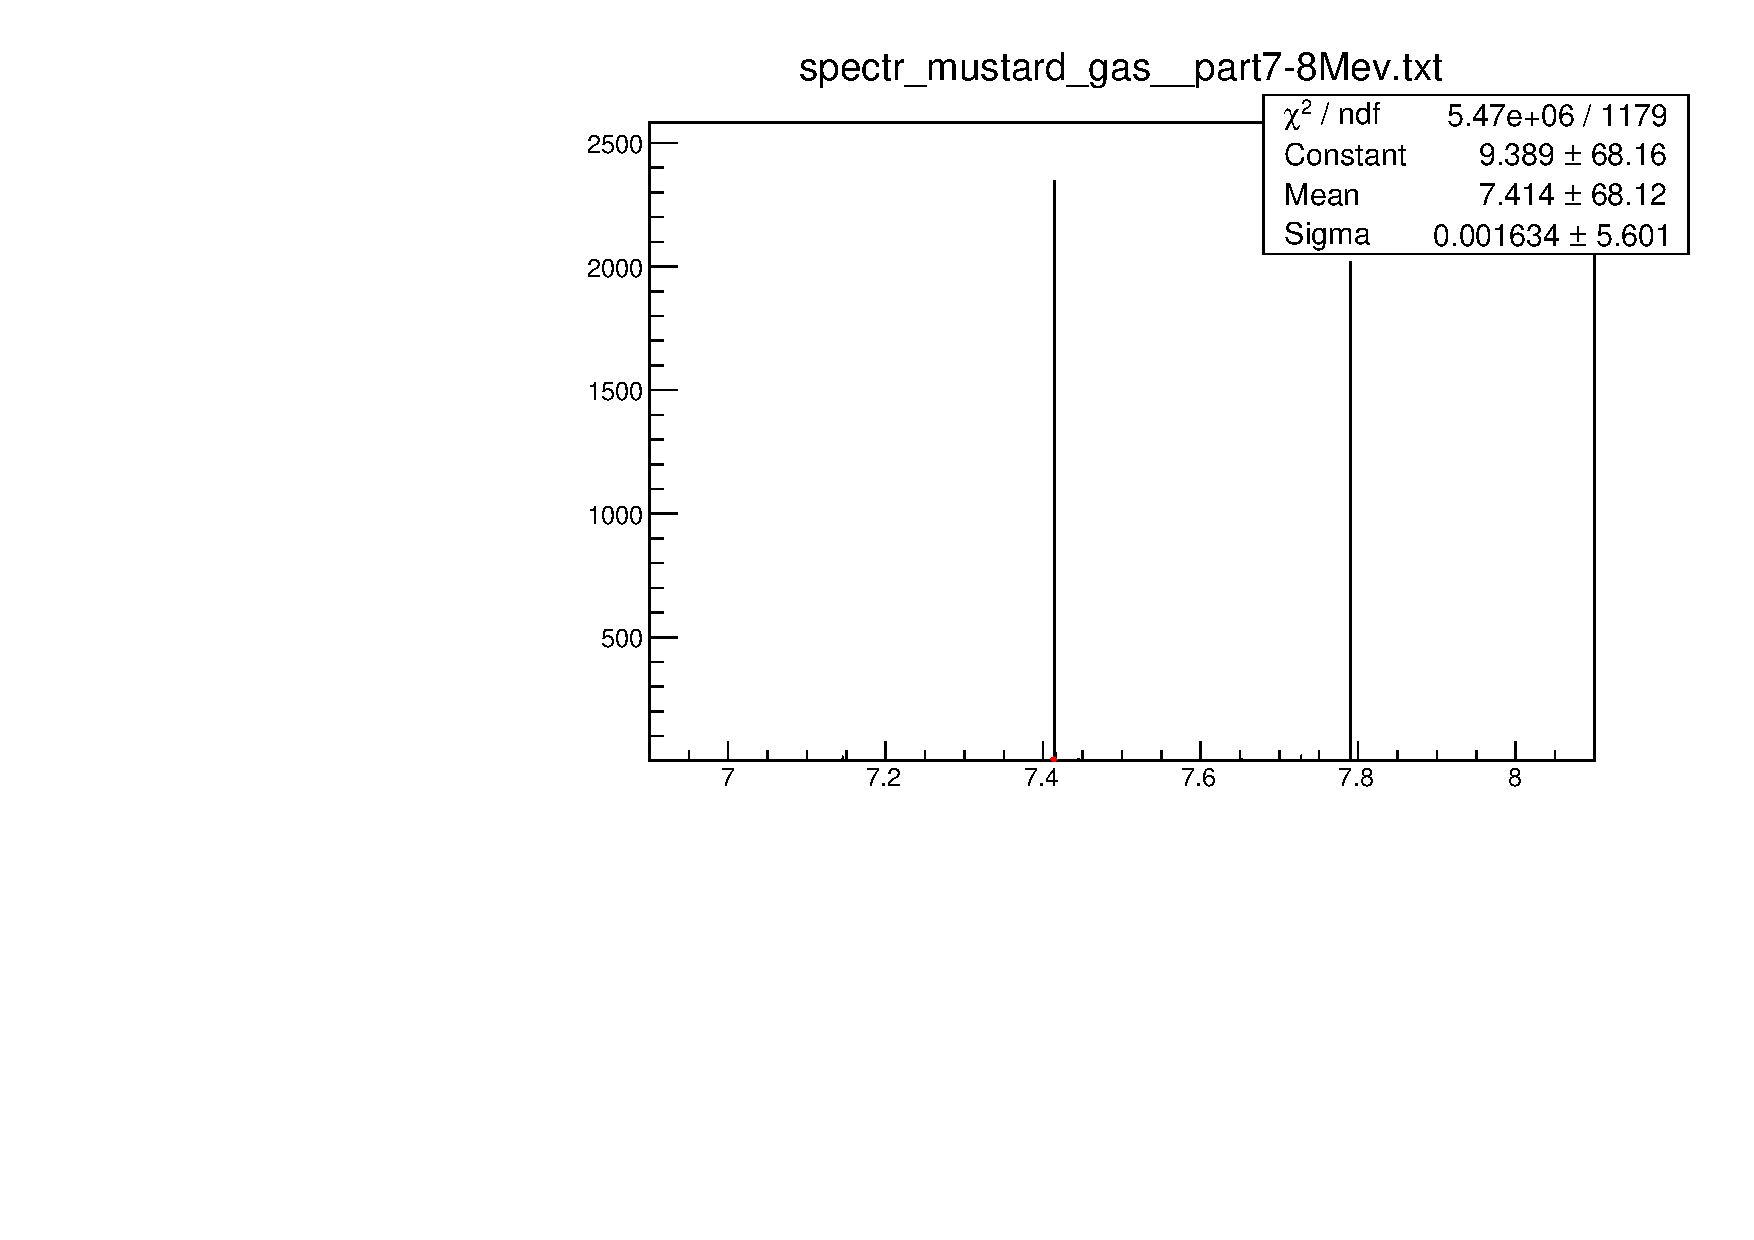
\includegraphics[width=1\textwidth]{Cl7_44MeV.pdf}
			\caption{Лінія яка відповідає 7.44 Mev Cl в проекті Сабат, червоним побудований гаусс}
			\label{ris:image7}
		\end{figure}

		\begin{figure}[hbt!]
			%\vspace{-10pt}
			\centering 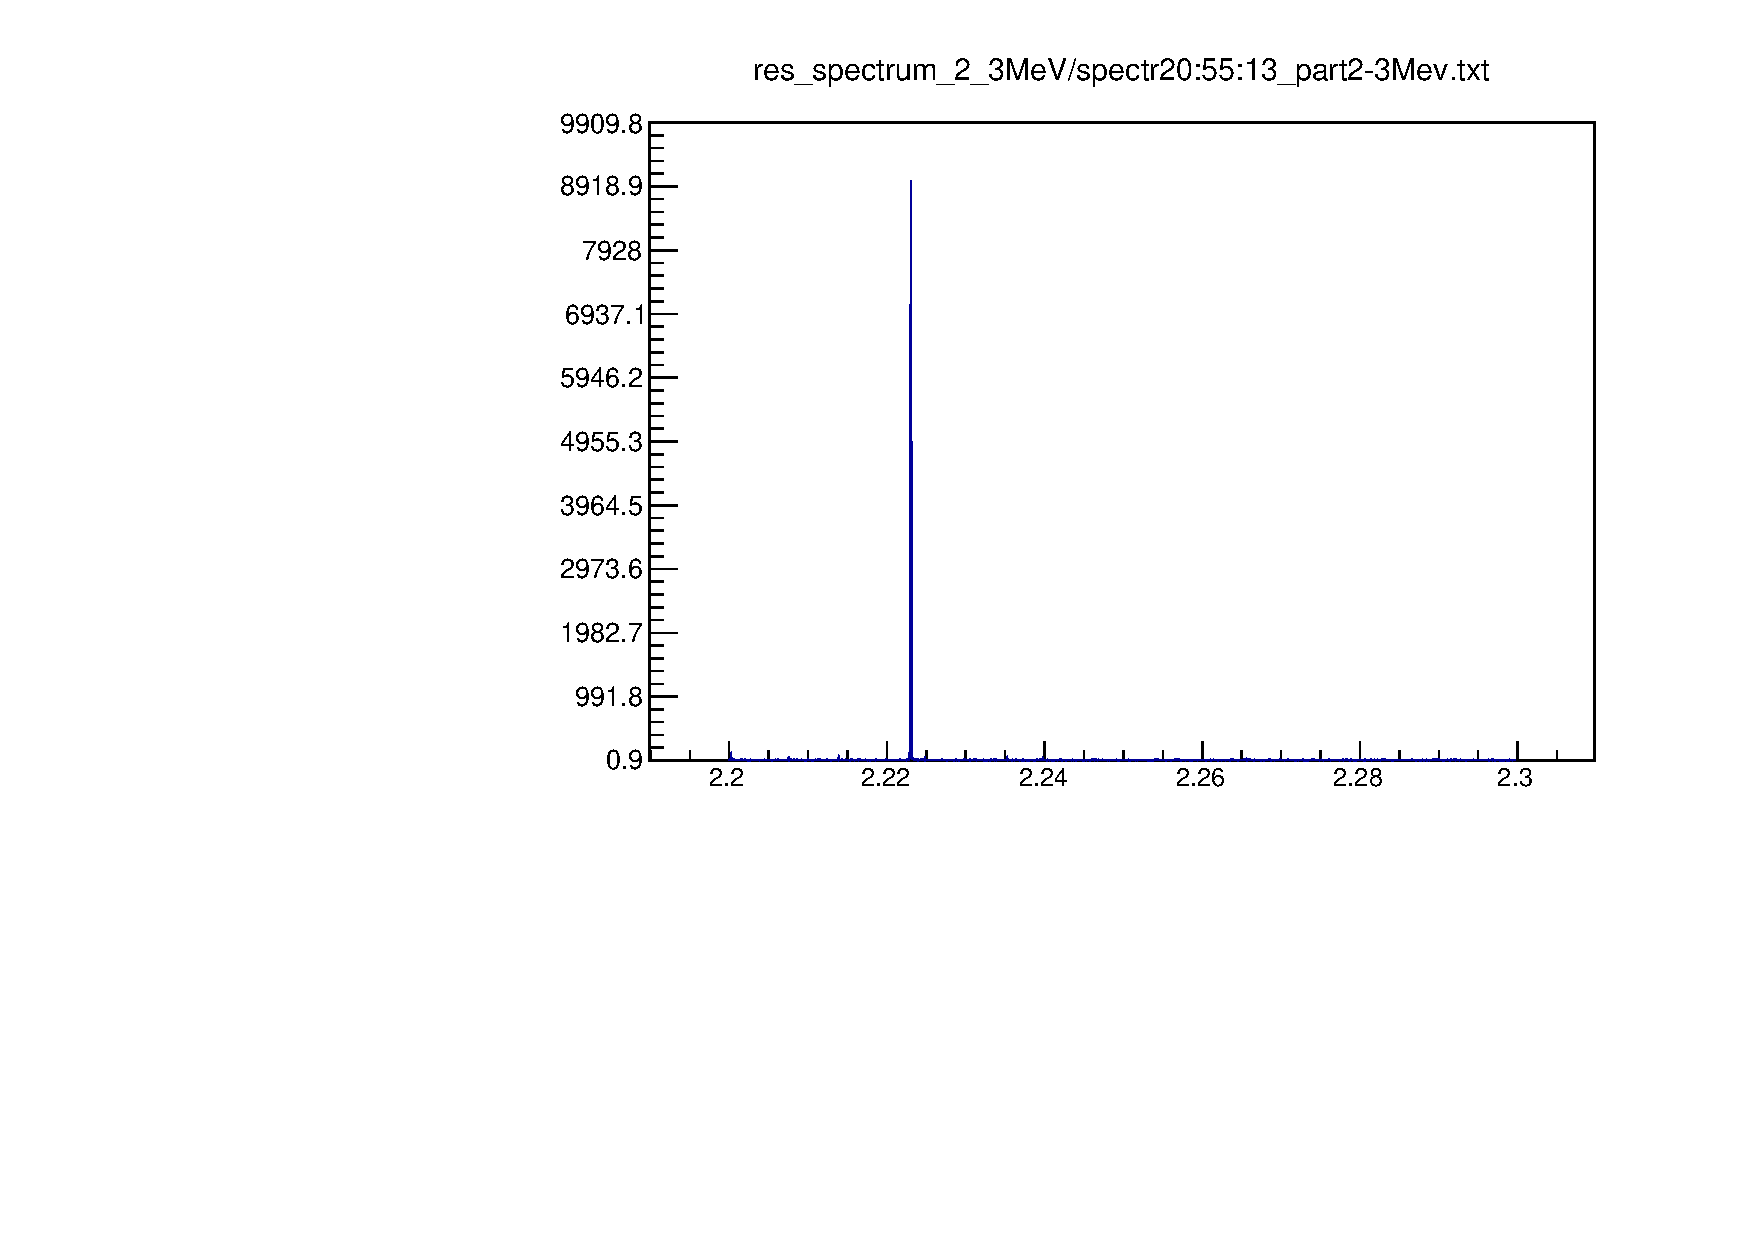
\includegraphics[width=1\textwidth]{2_3MeV.pdf}
			\caption{це частина спектру від 2.2 - 2.3 Mev}
			\label{ris:image7}
		\end{figure}
	
	Мені вдалося знайти всі лінії хлору, з проекту сабат 
	
	
\end{document}